\documentclass[aspectratio=169,11pt]{beamer}
\def\courseweek{7}
% Shared style for the Introduction to Information Geometry lecture slides.
% Compile the lecture .tex files from this directory.
\providecommand{\courseweek}{1}
\usepackage[T1]{fontenc}
\usepackage[utf8]{inputenc}
\usepackage[sc]{mathpazo}
\renewcommand{\sfdefault}{lmss}
\renewcommand{\ttdefault}{lmtt}
\usepackage{amsmath,amssymb,mathtools}
\usepackage{tikz}
\usetikzlibrary{arrows.meta,calc,positioning}
\usepackage{pgfplots}
\pgfplotsset{compat=1.18}
\usepackage{booktabs}

\definecolor{courseink}{HTML}{173749}
\definecolor{coursemuted}{HTML}{526674}
\definecolor{courseteal}{HTML}{0E7287}
\definecolor{coursecopper}{HTML}{B66B43}
\definecolor{courseline}{HTML}{D4E0E3}
\definecolor{coursepale}{HTML}{EFF5F5}

\setbeamercolor{normal text}{fg=courseink,bg=white}
\setbeamercolor{structure}{fg=courseteal}
\setbeamercolor{frametitle}{fg=courseink,bg=white}
\setbeamercolor{title}{fg=courseink}
\setbeamercolor{subtitle}{fg=coursemuted}
\setbeamercolor{block title}{fg=courseink,bg=white}
\setbeamercolor{block body}{fg=courseink,bg=white}
\setbeamercolor{alerted text}{fg=coursecopper}
\setbeamerfont{title}{family=\rmfamily,series=\bfseries,size=\fontsize{32}{37}}
\setbeamerfont{frametitle}{family=\rmfamily,series=\bfseries,size=\fontsize{26}{31}}
\setbeamerfont{normal text}{size=\fontsize{18}{22}}
\setbeamerfont{subtitle}{size=\fontsize{17}{21}}
\setbeamersize{text margin left=0.78cm,text margin right=0.78cm}
\setbeamertemplate{navigation symbols}{}
\setbeamertemplate{itemize items}[circle]
\setbeamertemplate{enumerate items}[default]
\setbeamertemplate{blocks}[default]
\setlength{\parskip}{0.22em}
\setbeamertemplate{footline}{%
  \leavevmode\hbox to \paperwidth{\hspace{.78cm}%
  {\color{coursemuted}\fontsize{8.5}{10}\selectfont Introduction to Information Geometry \hspace{.32cm} / \hspace{.32cm} Week \courseweek}%
  \hfill{\color{coursemuted}\fontsize{8.5}{10}\selectfont \insertframenumber\hspace{.17cm}/\hspace{.17cm}\inserttotalframenumber}\hspace{.78cm}}%
  \vskip.17cm
}
\setbeamertemplate{frametitle}{%
  \vspace{.13cm}
  \insertframetitle\par
  \vspace{.08cm}
}
\setbeamertemplate{title page}{%
  \vspace*{1.00cm}
  {\color{courseteal}\fontsize{10}{13}\selectfont\bfseries
  INTRODUCTION TO INFORMATION GEOMETRY\par}
  \vspace{.40cm}
  {\usebeamerfont{title}\usebeamercolor[fg]{title}\inserttitle\par}
  \vspace{.22cm}
  {\usebeamerfont{subtitle}\usebeamercolor[fg]{subtitle}\insertsubtitle\par}
  \vfill
  {\color{coursemuted}\fontsize{13}{16}\selectfont Christopher Lee\par}
  \vspace{.34cm}
}

\pgfplotsset{
  courseplot/.style={
    width=11.05cm,
    height=5.15cm,
    axis line style={coursemuted!75},
    tick style={coursemuted!65},
    ticklabel style={font=\scriptsize,color=coursemuted},
    label style={font=\normalsize,color=courseink},
    grid=major,
    major grid style={courseline!70,line width=.4pt},
    line width=1.45pt,
    legend style={font=\small,draw=none,fill=none,at={(.98,.03)},anchor=south east},
    clip=true
  }
}

\newcommand{\highlightmath}[1]{{\color{courseteal}#1}}
\newcommand{\thinrule}{\par\vspace{.25cm}{\color{courseline}\rule{\linewidth}{.8pt}}\par}

% A one-dimensional state space.  x=0 and x=1 are placed at 0 and 9 units.
\newcommand{\stateinterval}[1]{%
 \begin{tikzpicture}[x=1cm,y=1cm]
   \draw[courseink,line width=1.25pt] (0,0)--(9,0);
   \foreach \pos/\lab in {0/0,9/1} {
     \fill[courseink] (\pos,0) circle(2.7pt);
     \node[below=9pt,text=coursemuted] at (\pos,0) {\(\lab\)};
   }
   #1
 \end{tikzpicture}%
}

% Paired pages are separate frames in the PDF, with matching titles.
% Supply the whole frame body for each version; the instructor may edit them
% independently without changing overlay logic.
\newcommand{\coursepair}[3]{%
  \begin{frame}{#1}#2\end{frame}%
  \begin{frame}{#1}#3\end{frame}%
}

% Equilateral representation of the categorical simplex, in barycentric
% coordinates with vertices A=(0,0), B=(1,0), C=(1/2,sqrt(3)/2).
\newcommand{\coursesimplex}[1]{%
 \begin{tikzpicture}[scale=4.9]
  \fill[coursepale] (0,0)--(1,0)--(.5,.8660254)--cycle;
  \draw[courseink,line width=.65pt] (0,0)--(1,0)--(.5,.8660254)--cycle;
  \node[below left,font=\small] at (0,0) {A};
  \node[below right,font=\small] at (1,0) {B};
  \node[above,font=\small] at (.5,.8660254) {C};
  #1
 \end{tikzpicture}%
}

\title{Fisher Length and Replicator Speed}
\subtitle{Week 7 \(\cdot\) Lecture 2}
\date{}
\begin{document}
\begin{frame}[plain]\titlepage\end{frame}

\begin{frame}{Length of a curve of distributions}
For a differentiable path \(P(t)=(p_i(t))\), its Fisher speed is
\[
\|P'(t)\|_F=\sqrt{\sum_i\frac{(p_i'(t))^2}{p_i(t)}}.
\]
\vspace{.46cm}
Integrating gives its length:
\[
\highlightmath{L_F(P)=\int_a^b\|P'(t)\|_F\,dt}.
\]
\end{frame}

\begin{frame}{The Bernoulli line element}
For \(P_p=(p,1-p)\),
\[
\highlightmath{ds^2=\frac{dp^2}{p(1-p)}}.
\]
\vspace{.43cm}
The distance between \(p=a\) and \(p=b\) is
\[
d_F(a,b)=\left|\int_a^b\frac{dp}{\sqrt{p(1-p)}}\right|.
\]
\vspace{.39cm}
The metric's varying coefficient controls the accumulated length.
\end{frame}

\begin{frame}{An arc coordinate makes length constant}
Set \(p=\sin^2(\theta/2)\). Then
\[
dp=\frac12\sin\theta\,d\theta,
\qquad \sqrt{p(1-p)}=\frac12\sin\theta.
\]
\vspace{.48cm}
Thus \(ds^2=d\theta^2\), and
\[
\highlightmath{\theta(p)=2\arcsin\sqrt p}.
\]
\end{frame}

\coursepair{A Bernoulli Fisher distance}{
Use
\[
d_F(a,b)=2\left|\arcsin\sqrt b-\arcsin\sqrt a\right|.
\]
\vspace{.43cm}
Find the distance from \(a=\frac14\) to \(b=\frac34\).
}{
Use
\[
d_F(a,b)=2\left|\arcsin\sqrt b-\arcsin\sqrt a\right|.
\]
\vspace{.43cm}
The arc coordinates are \(\theta_a=\frac\pi3\) and
\(\theta_b=\frac{2\pi}3\). Therefore
\[
\highlightmath{d_F(\tfrac14,\tfrac34)=\frac\pi3}.
\]
}

\begin{frame}{The arc coordinate is nonlinear}
\vspace{-.2cm}
\begin{center}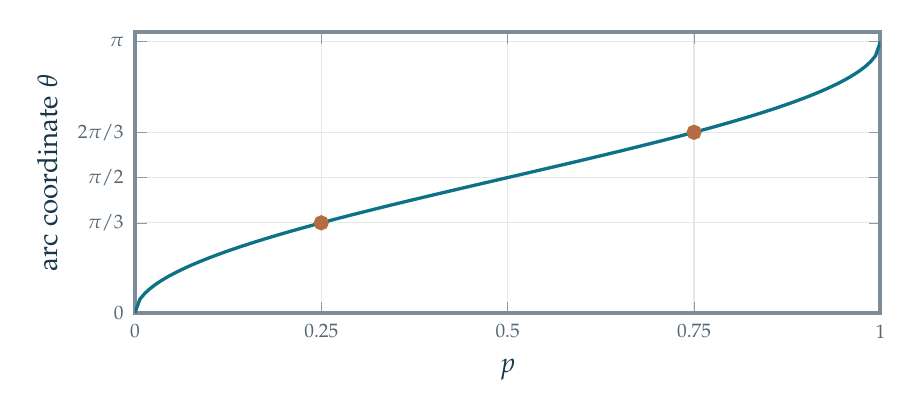
\begin{tikzpicture}
\begin{axis}[courseplot,xmin=0,xmax=1,ymin=0,ymax=3.25,
 xlabel={$p$},ylabel={arc coordinate $\theta$},
 xtick={0,.25,.5,.75,1},ytick={0,1.0472,1.5708,2.0944,3.14159},
 yticklabels={0,$\pi/3$,$\pi/2$,$2\pi/3$,$\pi$}]
\addplot[courseteal,very thick,domain=.00001:.99999,samples=150]
{2*asin(sqrt(x))*pi/180};
\addplot[only marks,coursecopper,mark=*,mark size=2pt]
coordinates{(.25,1.04719755)(.75,2.0943951)};
\end{axis}\end{tikzpicture}\end{center}
\end{frame}

\begin{frame}{The categorical Fisher matrix}
Let \(P=(x,y,z)\) with \(z=1-x-y\). Then \(dz=-dx-dy\), so
\[
ds^2=\frac{dx^2}{x}+\frac{dy^2}{y}+\frac{(dx+dy)^2}{z}.
\]
\vspace{.38cm}
In independent coordinates \((x,y)\),
\[
\highlightmath{G(x,y)=\begin{pmatrix}1/x+1/z&1/z\\1/z&1/y+1/z\end{pmatrix}}.
\]
\end{frame}

\coursepair{The metric at a categorical law}{
For \(P=(x,y,z)=(.2,.3,.5)\), compute
\[
G=\begin{pmatrix}1/x+1/z&1/z\\1/z&1/y+1/z\end{pmatrix}.
\]
\vspace{.45cm}
What are its three distinct entries?
}{
For \(P=(x,y,z)=(.2,.3,.5)\), compute
\[
G=\begin{pmatrix}1/x+1/z&1/z\\1/z&1/y+1/z\end{pmatrix}.
\]
\vspace{.45cm}
The result is
\[
\highlightmath{G=\begin{pmatrix}7&2\\2&16/3\end{pmatrix}}.
\]
}

\begin{frame}{Tangent velocity as a random variable}
At positive \(P\), assign a tangent vector \(v\) the values
\[
a_i=\frac{v_i}{p_i}.
\]
\vspace{.43cm}
Then \(E_P[a]=\sum_i v_i=0\), and
\[
\highlightmath{g_P(v,v)=E_P[a^2]=\operatorname{Var}_P(a)}.
\]
\vspace{.36cm}
Fisher norm is an ordinary variance when expressed in relative rates.
\end{frame}

\begin{frame}{Replicator velocities have a simple norm}
The replicator equation is
\[
p_i'=p_i(f_i-\bar f).
\]
\vspace{.45cm}
Its relative rate is \(p_i'/p_i=f_i-\bar f\). Hence
\[
\highlightmath{\|\mathbf p'\|_F^2
=\sum_i p_i(f_i-\bar f)^2
=\operatorname{Var}_{\mathbf p}(f)}.
\]
\end{frame}

\coursepair{The speed of a replicator state}{
At \(P=(.2,.3,.5)\), let \(f=(3,1,2)\).
\vspace{.43cm}
The mean fitness is \(\bar f=1.9\).
\vspace{.3cm}
Compute \(\|P'\|_F^2=\operatorname{Var}_P(f)\).
}{
At \(P=(.2,.3,.5)\), let \(f=(3,1,2)\).
\vspace{.43cm}
The fitness deviations are \((1.1,-.9,.1)\).
\[
\|P'\|_F^2=.2(1.1)^2+.3(-.9)^2+.5(.1)^2
=\highlightmath{.49}.
\]
\vspace{.17cm}
The Fisher speed is \(\highlightmath{.7}\).
}

\begin{frame}{Motion and geometry now use the same units}
The replicator equation supplies tangent vectors.
\vspace{.5cm}
Fisher information assigns lengths to those vectors.
\vspace{.5cm}
The next step is to find the shortest intrinsic paths
between two distributions. Their geometry becomes visible
after a square-root change of coordinates.
\end{frame}
\end{document}
